% mnras_template.tex
%
% LaTeX template for creating an MNRAS paper
%
% v3.0 released 14 May 2015
% (version numbers match those of mnras.cls)
%
% Copyright (C) Royal Astronomical Society 2015
% Authors:
% Keith T. Smith (Royal Astronomical Society)

% Change log
%
% v3.0 May 2015
%    Renamed to match the new package name
%    Version number matches mnras.cls
%    A few minor tweaks to wording
% v1.0 September 2013
%    Beta testing only - never publicly released
%    First version: a simple (ish) template for creating an MNRAS paper

%%%%%%%%%%%%%%%%%%%%%%%%%%%%%%%%%%%%%%%%%%%%%%%%%%
% Basic setup. Most papers should leave these options alone.
\documentclass[a4paper,fleqn,usenatbib]{mnras}

% MNRAS is set in Times font. If you don't have this installed (most LaTeX
% installations will be fine) or prefer the old Computer Modern fonts, comment
% out the following line
\usepackage{newtxtext,newtxmath}

% Depending on your LaTeX fonts installation, you might get better results with one of these:
%\usepackage{mathptmx}
%\usepackage{txfonts}

% Use vector fonts, so it zooms properly in on-screen viewing software
% Don't change these lines unless you know what you are doing
\usepackage[T1]{fontenc}
\usepackage{ae,aecompl}


%%%%% AUTHORS - PLACE YOUR OWN PACKAGES HERE %%%%%

% Only include extra packages if you really need them. Common packages are:
\usepackage{graphicx}	% Including figure files
\usepackage{amsmath}	% Advanced maths commands
\usepackage{amssymb}	% Extra maths symbols

\usepackage{xspace}

%%%%%%%%%%%%%%%%%%%%%%%%%%%%%%%%%%%%%%%%%%%%%%%%%%

%%%%% AUTHORS - PLACE YOUR OWN COMMANDS HERE %%%%%

% Please keep new commands to a minimum, and use \newcommand not \def to avoid
% overwriting existing commands. Example:
%\newcommand{\pcm}{\,cm$^{-2}$}	% per cm-squared

%%%%%%%%%%%%%%%%%%%%%%%%%%%%%%%%%%%%%%%%%%%%%%%%%%

\def\ngradeA{13}
\def\ngradeB{23}
\def\ngradeC{175}

\def\Sref#1{Section~\ref{#1}\xspace}
\def\Fref#1{Figure~\ref{#1}\xspace}
\def\Tref#1{Table~\ref{#1}\xspace}
\def\Eref#1{Equation~\ref{#1}\xspace}

\def\pr{{\rm Pr}}
\def\plens{\pr_{\mathrm{lens}}}

\def\thetae{\theta_{\mathrm{E}}}

\usepackage[usenames]{color}
\newcommand{\comment}[2]{\textcolor{red}{\textbf{QUERY (#1): #2}}}

%%%%%%%%%%%%%%%%%%% TITLE PAGE %%%%%%%%%%%%%%%%%%%

% Title of the paper, and the short title which is used in the headers.
% Keep the title short and informative.
\title[]{SUGOHI I: automatic search for strong lenses in the HSC survey}

% The list of authors, and the short list which is used in the headers.
% If you need two or more lines of authors, add an extra line using \newauthor
\author[A. Sonnenfeld et al.]{
Alessandro Sonnenfeld,$^{1}$\thanks{E-mail: alessandro.sonnenfeld@ipmu.jp}
Anupreeta More,$^{1}$
Masamune Oguri,$^{1,2}$
Yiping Shu,$^{3}$\newauthor
Sherry H. Suyu,$^{4}$
James H. H. Chan,$^{5}$
Kenneth C. Wong,$^{6}$
\\
% List of institutions
$^{1}$Kavli IPMU (WPI), UTIAS, The University of Tokyo, Kashiwa, Chiba 277-8583, Japan \\
$^{2}$Department of Physics, University of Tokyo, 7-3-1 Hongo, Bunkyo-ku, Tokyo 113-0033, Japan \\
$^{3}$National Astronomical Observatories, Chinese Academy of
Sciences, 20A Datun Road, Chaoyang District, Beijing 100012,
China \\
$^{4}$1Max-Planck-Institut fur Astrophysik, Karl-Schwarzschild-Str. 1, 85748 Garching, Germany \\
$^{5}$Department of Physics, National Taiwan University, 10617 Taipei, Taiwan
$^{6}$National Astronomical Observatory of Japan, 2-21-1 Osawa, Mitaka, Tokyo 181-8588, Japan
}
% These dates will be filled out by the publisher
\date{Accepted XXX. Received YYY; in original form ZZZ}

% Enter the current year, for the copyright statements etc.
\pubyear{2016}

% Don't change these lines
\begin{document}
\label{firstpage}
\pagerange{\pageref{firstpage}--\pageref{lastpage}}
\maketitle

% Abstract of the paper
\begin{abstract}
We developed a method to look for galaxy-scale strong gravitational lenses in photometric data. We applied it to the first internal data release of the HSC SSP survey. We found $\ngradeA$ definite lenses, $\ngradeB$ highly probable lenses and $\ngradeC$ possible lenses.
\end{abstract}

% Select between one and six entries from the list of approved keywords.
% Don't make up new ones.
\begin{keywords}
keyword1 -- keyword2 -- keyword3
\end{keywords}

%%%%%%%%%%%%%%%%%%%%%%%%%%%%%%%%%%%%%%%%%%%%%%%%%%

%%%%%%%%%%%%%%%%% BODY OF PAPER %%%%%%%%%%%%%%%%%%

\section{Introduction}

Lenses are great.

\section{The Data}

\subsection{HSC photometry}
The HSC survey is great.

We used photometric data in the $i$ and $g$ band from the 2016A data release of the Wide compoent of the HSC survey.

\subsection{BOSS spectroscopy and target selection}

Our strong lens search is lens-based: we select objects with characteristic properties of lens galaxies and then look for the presence of lensed background sources.
We select lens galaxy candidates from the Baryon Oscillation Spectroscopic Survey \citep[BOSS][]{SWE09}
The BOSS survey consists of two subsamples of luminous red galaxies (LRGs): the LOWZ and CMASS samples. The main difference between the two samples is mostly the redshift distribution: LOWZ galaxies are mostly at $z < 0.4$ while CMASS galaxies are mostly in the range $0.4 < z < 0.7$.
The number of BOSS galaxies with HSC photometry in the 2016A data release is XXX, of which YYY from LOWZ and ZZZ from CMASS.

There are two reasons for selecting lens galaxy candidates from the BOSS survey. Firstly, BOSS targeted the high mass end of the galaxy population. Since the strong lensing cross section increases with lens mass, more massive galaxies are more likely to be lenses.
Secondly, optical spectroscopy data from BOSS allows us to look for signatures from strongly lensed star forming galaxies in the form of emission lines at a different redshift from the lens.
The detection of emission lines from the background galaxy can add crucial information for the classification of a lens candidate. Moreover, a spectroscopic measurement of the redshift of both the lens and source galaxy allows us to convert angular measurements of the Einstein radius into mass measurements.

\section{The Method}

YattaLens, our lens finding algorithm, consists of several steps, each described in detail below.
The basic idea can be summarized in two key points: 1) YattaLens looks for arc-like features around massive galaxies and 2) fits simple lens models to these arcs to assess the likelihood of them being lensed galaxies.
The first step is smilar to other existing lens finding algorithms, such as ARCFINDER \citep{Ala06, Mor++12} or RINGFINDER \citep{Gav++14}, while the second step shares similarities with the lens finding method of \citet{Mar++09}.
The details in which these two steps are implemented in YattaLens however are different from the methods listed above.

There are several challenges in the search for galaxy-scale lenses in ground-based imaging data.
First of all, for many strong lenses the Einstein radius, roughly the mean distance of lensed images from the center of the lens, is on the order of the half-light radius of the lens. This means that lensed images are often blended with the surface brightness of the foreground galaxy, making their detection more complicated.
Secondly, as we will show later, many non-lenses exhibit arc-like features due to the presence of spiral arms or tangentially elongated star forming regions,  increasing the risk of false-positive detection.
Thirdly, lens galaxies are often times surrounded by satellites, companions, or unrelated objects in close proximity on the line of sight. This complicates the identification of lensed images.
YattaLens is designed to tackle these challenges.

\subsection{Lens Light subtraction}

The first step in the search for lensed arcs consists in removing from the image the contribution from the candidate lens galaxy.
We do this by fitting an elliptical de Vaucouleurs surface brightness profile \citep{deV48} to the $i$-band data in a small (3'' radius) region around the center of the galaxy. 
This step takes a few seconds on a normal machine.
We choose the $i$-band for two reasons: 1) the image quality of HSC data is best in this band and 2) we expect the lens galaxy to outshine lensed background galaxies at this wavelength, since typical lens systems consist of a massive red galaxy in the foreground and a blue star-forming galaxy in the background.

We then take the best fit de Vaucouleurs model and subtract a PSF-convolved, rescaled version of it from the $i$-band and all other bands used in the analysis (in our case the $g$-band). 
With this step we are implicitly assuming that there are no color gradients in the lens galaxy.

Examples of lens-subtracted images are shown in the second column of \Fref{fig:examples1}.

\subsection{Lensed arc identification}\label{ssec:arc}

We use SExtractor to look for objects in the lens-subtracted $g$-band image.
For each object we consider their position relative to the lens light centroid, their axis ratio and orientation, the size of their footprint. 

%and their $g-i$ color. The color is estimated by simply measuring the $g$ and $i$-band flux in the $g$-band footprint. Although in principle differences in the PSF between the two bands can affect the color estimated in this way, we do not require high accuracy and do not attempt to match the PSF in this step.

We then apply the following series of conditions to determine whether an object can be a lensed arc or not.
%
\begin{enumerate}
%\item A maximum $g-i$ color of 2.0.
\item A distance from the lens centroid between 3 and 30 pixels ($0.50'' < R < 5.04''$)
\item A minimum ratio between the major and minor axis of 1.4
\item A maximum difference of 30 degrees between the position angle of the major axis of the object and the tangential to the circle centered on the lens and passing through the object centroid.
\item A minimum angular aperture, defined as the angle subtended by the object from the lens centroid, of 25 degrees.
\item A footprint size between 20 and 500 pixels.
\end{enumerate}
%
%Condition 1 requires the arc candidate to be relatively blue. Although a $g-i$ color of 2.0 is not a particularly strong limit, it is sufficient to eliminate a frequent source of contaminants: satellite galaxies with major axis oriented along the tangential direction.
The minimum distance requirement in condition (i), as well as the minimum size requirement in condition (v), makes sure that the candidate arc is not just a residual from a non-perfect subtraction of the lens light. The maximum distance constraint is applied because we do not expect galaxy scale lenses to have Einstein radii larger than $5''$. Although there are lenses with larger Einstein radius, we typically refer to these as group-scale or cluster-scale lenses.
Conditions (ii) and (iii) are applied to only select tangentially elongated objects.
We add condition (iv) to select objects that are elongated not just in terms of axis ratio but that also describe a sizeable arc around the lens, in angular terms. This conditions eliminates small objects far away from the lens that happen to pass the orientation and axis ratio requirement given by condition (ii) and (iii) but are clearly not strongly lensed.
Finally we add the maximum size requirement in condition (v) to reject catastrophic failures in the object detection process.
Objects that pass all five conditions are kept as potential arcs.

\subsection{Foreground model}\label{ssec:foreground}

If the object detection process described above returned at least one arc candidate, we proceed with a more accurate fit of the lens light and by modeling potential foreground objects.
We turn back to the $i$-band data and fit a S\'{e}rsic profile \citep{Ser68} to the surface brightness distribution of the main galaxy, this time masking out any objects detected in the $g$-band image by SExtractor.
We then go through non-arc-like objects detected in the $i$-band around the lens, one by one in order of decreasing $i$-band flux, and fit each one with a S\'{e}rsic profile.Each time a new object is fit, the structural parameters of the lens and previously fitted objects (i.e. centroid, effective radius, etc.) are kept fixed, as well as the relative $i$-band amplitude between the lens and any other object fit up to that point. Only the overall amplitude of all previously fit objects is varied. 
This prescription is adopted to reduce computation time.
Only objects within $1.4$ times the distance of the farthest arc candidate of the lens are modeled. Objects farther away are simply masked out.%, since they are to far to be counter-images to the main arc.

Although most known lenses do not have foreground objects other than the lens galaxy itself in the proximity of lensed images, accounting for the presence of foregrounds is important for the rejection of false positive candidates.
An example of foreground object modeling is shown in the first row of \Fref{fig:examples1}. After the lens light subtraction step, a galaxy is detected North of the lens and is then modeled with a S\'{e}rsic profile. The model of the lens and foreground object, together with a model for the lensed source to be described in \ref{ssec:lens}, is shown in the fourth column.

Up to this point, no color information has been used. Among the objects treated as foreground there might be counter-images of the main arc. In the next subsection we will illustrate how we can classify images based on their color.

%In \Fref{fig:fgmodel} we show an example of all the steps described so far: lens subtraction, search for arcs, detection 


\subsection{Multiple image set candidates}

At this stage of the lens finding process we have candidate arcs and a model for the light distribution of the lens galaxy and surrounding objects.
These objects can be either foregrounds or multiple images of the arcs.
We use color and position information to distinguish between the two possibilities.

First of all we apply a color selection to the arc candidates themselves. Since we expect lensed galaxies to be relatively blue we require a $g-i$ color smaller than $2.0$.
Although a $g-i$ color of $2.0$ is not a particularly strong limit, it is sufficient to eliminate a frequent source of contaminants: satellite galaxies with major axis oriented along the tangential direction.
In principle this color selection criterion could have been applied before the foreground object modeling step, in the interest of time. However, having an accurate model for the system is important to measure accurate colors and avoid rejecting good lenses for which the light from the arc happens to be contaminated by a foreground object.
 
We then go through the blue (according to our color cut) arcs and create sets of arcs and non-arc objects with consistent $g-i$ color, which we interpret as candidate sets of multiple images of the same source. 
We require colors of different objects to be within $2-\sigma$ of each other in order to consider them consistent. To take into account modeling systematics we add in quadrature to the statistical uncertainty on the flux of individual pixels a systematic uncertainty equal to 20\% of the flux of the best fit model of lens and foregrounds.

The minimal multiple image set consists of only one arc. 
If other candidate arcs are present and if they have consistent $g-i$ color they are added to the set. An example of such a case is shown in the second row of \Fref{fig:examples1}: two objects satisfying the definition of arc given in \ref{ssec:arc} are found by running SExtractor on the lens-subtracted image, shown in bright green in the segmentation map panel (third column). Since they have consistent colors, they are interpreted as multiple imges of the same source.

If on the contrary there are arc-like objects with a different color than the arc defining the set, and if they are within 1.3 times the distance of the farthest arc from the lens, they are classified as foreground and are fitted with a S\'{e}rsic profile with the same procedure described in \ref{ssec:foreground}. If these arc-like objects are at a farther distance from the lens they are simply masked out.
An example of this process is shown in the third and fourth row of \Fref{fig:examples1}. For this lens candidate, our algorithm led to the detection of two potential arcs: an extended blue arc to the North-West of the main galaxy and a redder object to the East.
Both objects could be lensed sources, but since they have different colors they cannot be multiple images of the same object. Then, two different interpretations are possible. If the bluer, bigger arc is the lensed source, then the red object must be a foreground. Since this object is too far away from the lens galaxy to affect any further analysis, it is simply masked out. This scenario is shown in the third row: the candidate arc is shown in bright green and objects masked out are shown in red.
In the fourth row, the second interpretation is illustrated: the redder object is considered to be the lensed source, and the bluer elongated feature is modeled as a foreground (marked in white in the segmentation map plot).

Finally we repeat the same procedure for non-arc-like objects: those with color consistent with the candidate arc(s) are assigned to a multiple image set. Objects with a different color are either modeled as foregrounds or masked out, depending on their distance from the lens galaxy.
In the same system discussed above, a faint object is detected South of the lens. This is masked out in the first interpretation of the image configuration (third row of \Fref{fig:examples1}, but is instead modeled as a foreground in the second interpretation (fourth row), because its distance from the lens is within 1.3 times that of the main arc.

In the fifth row we show an instance of a system in which a non-arc-like object with color consistent to a candidate arc is found. The object is represented in dark green in the segmentation map plot.
This object was modeled as a foreground in the previous step. However, since it is now treated as a counter-image of the arc, it is removed from the model of the foregrounds.

\subsection{Lens model}\label{ssec:lens}

We proceed to fit a lens model to each set of arcs and counter-images.
The lens mass model consists of a spherical isothermal ellipsoid, while the source surface brightness distribution is modeled with as a circularly symmetric exponential profile.
The centroid of the lens mass distribution is kept fixed to the value of the lens light centroid.
The free parameters of the model then are: lens angular Einstein radius $\thetae$, axis ratio $q$, position angle PA, source position $(s_x, s_y)$, source effective radius $s_e$, as well as the amplitude of the source, lens and foreground surface brightness components. 
We use a modified version of the lens modeling code developed by \citet{Aug++11} to find a maximum-likelihood fit to the data.
We explore the parameter space defined by the six non-linear parameters $\thetae$, $q$, PA, $s_x$, $s_y$ and $s_e$ with a Monte Carlo Markov Chain (MCMC), where at each step of the chain we optimize for the amplitudes of the surface brightness components.
We use the Python package {\em emcee} to sample the posterior probability distribution of the model parameters assuming flat priors on all of them.

This step of the algorithm is particularly slow. In order to minimize the cost in terms of time we only run a relatively short chain, without ensuring that the MCMC has converged and that the true maximum likelihood model has been found.
In order to maximize the chances of obtaining a good fit it is then important to find a reasonable starting solution.
We use the following prescription to define our starting model. We set the initial mass orientation and axis ratio equal to that of the light distribution. Then, in case only one arc is present, we assume that the Einstein radius is equal to $0.7$ times the distance of the arc from the lens. In case there are two or more arcs, the Einstein radius is set to the mean distance of the arcs from the lens.
Once the lens mass parameters are set, the starting position of the source is found by mapping each arc centroid to the source plane and taking the mean of their position.
We use the $g$-band image to perform the fit, since the contamination of the lensed images from the light of the lens galaxy and of typical foreground objects is lowest at this wavelength.

We then need to assess whether the best-fit lens model is a good description of the data. In principle we could use the $\xi^2$ to quantify the goodness-of-fit.
In practice, with our simple model it is almost impossible to fit the image of a lens down to noise level, let alone doing it automatically without human intervention.
Therefore, instead of considering absolute values of the $\chi^2$, which have little meaning, we compare the lens model $\chi^2$ with that obtained by fitting alternative models, described below.
%
\begin{figure*}
 \includegraphics[width=\textwidth]{example1.eps}
 \label{fig:examples1}
  \caption{Steps of the lens finding algorithm for a few example lenses and lens candidates. 
The first column shows the $gri$ image of the system. 
The second column contains a lens-subtracted image, displayed with a different contrast to enhance features from lensed objects. 
The third column shows a segmentation map plot of the objects identified by SExtractor. Green areas represent candidate arcs. Red areas are objects masked out. White areas are objects that are modeled as foreground, while dark green areas (only present in the fifth row) identify candidate counter-images to the main arc. 
The fourth column shows the best fit lens model of the system, including models for foreground objects. 
The fifth column shows the best model of the lensed background galaxy alone, with the contrast set equal to the second column. 
The sixth column shows the residuals between the data and the best-fit lens model.
The seventh and eight columns show the best fit ring and S\'{e}rsic models respectively. 
The numbers at the bottom of the images in column five, six and seven are the $\chi^2$ of the best fit model for the lens, ring and S\'{e}rsic model respectively.
Green circles in the top left corner of each row indicate candidates that passed the selection.
The red cross in the fourth row indicates that the second interpretation of the image configuration for the lens candidate HSCJ144428-005142 does not provide a good description of the system, since a model with a single S\'{e}rsic component at the position of the candidate arc gives a better fit.
Even though the images are color-composite, only the $g$-band is used for the modeling of the arc-like features.
The systems shown in rows a), b) and e) are known lenses from the SL2S survey \citep{Mor++12, Son++13a}. The system in rows c) and d) is a new candidate found in HSC data. The two different rows correspond to two different interpretations of the iamge configuration. In row c), the blue extended object is assumed to be the main arc (displayed in bright green color in the segmentation map). In row d) instead a different object is assumed to be the image of a lensed source, and the elongated blue feature is treated as a foreground object.
}
\end{figure*}
%

\subsection{Non-lens models}\label{ssec:nonlens}

The lens candidates that have made it thus far are systems with a relatively blue, tangentially elongated object close to a massive galaxy.
While some of these objects are indeed lenses, most of them are not.
The two main sources of contaminants are 1) spiral arms (we will use the term spiral arm in a broad sense to indicate a mostly tangentially elongated star forming region) and 2) foreground galaxies with high ellipticity.
The non-lens models that we compare against the lens model are designed to describe these two classes of systems.

The first model we consider is a ``ring galaxy'' model.
Its surface brightness profile is defined as follows
\begin{equation}\label{eq:ring}
I(r) = I_0 \left\{\begin{array}{ll} \exp{\{-(r-r_0)/h_o\}} & \rm{for}\,r>r_0 \\
\exp{\{-(r_0 - r)/h_i\}} & \rm{for}\,r<r_0\end{array}\right.
\end{equation}
Here $r$ is the circularized radius of elliptical isophotes,
\begin{equation}
r^2 \equiv qx^2 + y^2/q,
\end{equation}
and $r_0$, $h_i$ and $h_o$ are free parameters describing the radial position of the peak in the surface brightness distribution and an inner and outer scale radius, respectively.
The other free parameters of the model are the ellipticity $q$ and the position angle of the major axis, $\rm{PA}$.

Different realizations of a ring profile are shown in the seventh column of \Fref{fig:examples1}.
While our lens model cannot produce radially elongated images, due to the upper limit on source size and the choice of a singular isothermal profile, the ring model has the ability of describing relatively large regions with approximately constant surface brightness. For example, for very large values of the inner scale radius $r_i$, the ring profiles reduces to a disk with approximately constant surface brightness within $r_0$. 
Although hardly any galaxy can be well described by this surface brightness profile, the ring model provides a better fit compared to a lens model for most spiral galaxies that happen to be detected by the arc-finding step described in \ref{ssec:arc}, because it can provide a very rough description of their disk.
An example of a galaxy with a candidate arc for which a ring model gives a better fit compared to a lens model is shown in \Fref{fig:fail}.

When fitted to an actual lens, the ring model can hardly provide a reasonable fit. This is because the ring model is elliptically symmetric by construction, while the image configuration of strong lenses is not. The only case in which a ring profile could mimick a lens would be that of a perfectly circular Einstein ring. However a perfect Einstein ring requires both a perfectly circular mass distribution and a perfect alignment between lens and source, an extremely rare circumstance.

The second non-lens model that we fit is an S\'{e}rsic profile with disky/boxy isophotes. 
Many arc candidates picked by the algorithm are just foreground objects with relatively high ellipticity that happen to be tangentially aligned with respect to the lens.
A S\'{e}rsic profile provides a better fit with respect to a lens model for most of these systems.
One such example is shown in \Fref{fig:fail}, while another instance appears in the fourth row of \Fref{fig:examples1}, where the object interpreted as an arc is better fit by a S\'{e}rsic component.
%
\begin{figure}
 \includegraphics[width=\columnwidth]{failfig.eps}
 \label{fig:fail}
  \caption{Lens candidates rejected by our algorithm because a ring (top panel) or a S\'{e}rsic (bottom panel) model provides a better fit compared to a lens model. The top row shows a $gri$ image of the system, a lens-subtracted imaged and a segmentation map showing the footprint of the identified candidate arc (in bright green) and that of masked out object (in red).
The second row shows the best-fit lens model of the system, the corresponding source-only image and the residual.
The third row in the top (bottom) panel shows the best-fit ring (S\'{e}rsic) model, a ring-only (S\'{e}rsic-only) image and the residual.
}
\end{figure}


\subsection{A summary of the algorithm}

We have described in detail all the steps taken by YattaLens to look for strong lenses. Let us summarize the steps of the algorithm. 
\begin{enumerate}
\item Given a massive galaxy, YattaLens fits a S\'{e}rsic profile to its $i$-band surface brightness profile, then subtracts the best fit model from the $g$-band image 
\item Runs SExtractor on the lens-subtracted $g$-band image to look for tangentially elongated objects within $\sim5''$. 
\item If a candidate arc is found, YattaLens proceeds to model any object within a region where potential counter-images of the arc could be, then measures colors of arcs and other objects.
\item If the candidate arc is bluer than $g-i=2$, YattaLens makes sets of arcs and images of consistent color. For each multiple image set, any other object with inconsistent color is either modeled as a foreground object or masked out, depending on the ratio between its distance from the lens and the distance of the farthest candidate arc from the lesn.
\item For each multiple image set, the $g$-band image is fit with a lens model, a ring model and a S\'{e}rsic model. Each model includes a model of the lens galaxy and possible foreground objects, described as the sum of S\'{e}rsic profiles with fixed relative amplitude.
\item If the lens model provides a better fit, in terms of $\chi^2$, with respect to both the ring and the S\'{e}rsic model, the candidate is selected. Otherwise it is rejected.
\end{enumerate}
In the next subsection we will show how YattaLens performs on a sample of known lenses.

\subsection{Tests on known lenses}

The YattaLens algorithm has been tested and its parameters optimized on a sample of known lenses that lie in the 16A data release of HSC. These are 16 galaxy-scale lenses from the SL2S survey \citep[][SL2SJ021247-055552, SL2SJ021411-040502, SL2SJ021737-051329, SL2SJ022357-065142, SL2SJ022511-045433, SL2SJ022610-042011, SL2SJ022648-040610, SL2SJ022708-065445, SL2SJ023251-040823, SL2SJ023307-043838, SL2SJ090407-005952, SL2SJ142003+523137, SL2SJ220329+020518, SL2SJ220506+014703, SL2SJ221326-000946, SL2SJ222148+011542]{Gav++12, Son++13a, Son++15}, plus the double source plane lens HSCJ142449-005322 also known as the ``Eye of Horus'' \citep{Tan++16}.

YattaLens was able to identify correctly 15 lenses out of 17. The two systems missed by YattaLens are SL2SJ022357-065142 and SL2SJ022708-065445. Both were missed during the arc detection step, the arcs being too faint to be picked out by SExtractor, which we run with a detection threshold of $2-\sigma$ above the background.
The images of these two lenses, which were originally discovered using RINGFINDER \citep{Gav++14}, are shown in \Fref{fig:missed}.
In \Fref{fig:horus} we show how YattaLens' analysis on the double source plane lens The Eye of Horus.
Double source plane lenses are very interesting objects because they offer more constraints with respect to typical lenses and can be used for detailed studies of the mass distribution of the foreground galaxy \citep[e.g.][]{Son++12} or to infer cosmological parameters \citep{C+A14}.
Since they are also very rare, it is extremely important that lens finding algorithms do recognize them as lenses. This can be challenging for automatic algorithms because the presence of arcs from more than one source complicate their morphology.
Therefore we made sure when designing YattaLens that it could properly classify the Eye of Horus, the only double source plane lens known in the HSC survey \comment{AS}{Is that true, Anu??}, as a lens.

\section{The photometrically selected sample}

\subsection{Candidate grading}
We graded lens candidates output by YattaLens according to their likelihood of being strong lenses, $\plens$, using the following scheme:
\begin{itemize}
\item Grade A: definite lenses ($\plens > 0.997$), 
\item Grade B: probable lenses ($0.5 < \plens < 0.997$)
\item Grade C: possible lenses ($0.003 < \plens < 0.5$)
\item Grade 0: non lenses ($plens < 0.003$)
\end{itemize}

\section{The spectroscopically selected sample}

\section{Results}
In \Fref{fig:gradeA} we show the grade A lenses.
%
\begin{figure*}
 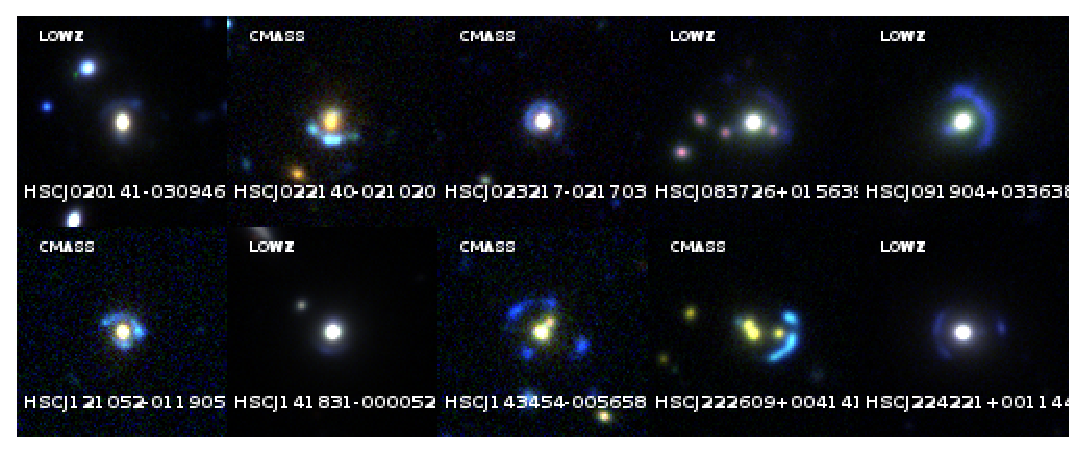
\includegraphics[width=\textwidth]{gradeA_collage.eps}
 \caption{Grade A lenses.}
 \label{fig:gradeA}
\end{figure*}
%
%
\begin{figure*}
 \includegraphics[width=\textwidth]{gradeB_collage.eps}
 \caption{Grade B lenses.}
 \label{fig:gradeA}
\end{figure*}
%
\section{Discussion}

\subsection{Lenses missed by YattaLens}

\subsection{Comparison with other lens samples}

\section{Conclusions}

\section*{Acknowledgements}

Acknowledgements.

%%%%%%%%%%%%%%%%%%%%%%%%%%%%%%%%%%%%%%%%%%%%%%%%%%

%%%%%%%%%%%%%%%%%%%% REFERENCES %%%%%%%%%%%%%%%%%%

% The best way to enter references is to use BibTeX:

%\bibliographystyle{mnras}
%\bibliography{example} % if your bibtex file is called example.bib
\bibliographystyle{mnras}
\bibliography{references}

%%%%%%%%%%%%%%%%%%%%%%%%%%%%%%%%%%%%%%%%%%%%%%%%%%

%%%%%%%%%%%%%%%%% APPENDICES %%%%%%%%%%%%%%%%%%%%%

% Don't change these lines
\bsp	% typesetting comment
\label{lastpage}
\end{document}

% End of mnras_template.tex
